\documentclass{article}
\usepackage[T2A]{fontenc}
\usepackage[utf8]{inputenc}
\usepackage[english,russian]{babel}
\usepackage{amssymb,amsfonts,amsmath,mathtext, wasysym}
\usepackage{cite,enumerate,float,indentfirst}
\usepackage[left=3cm,right=3cm,top=1cm,bottom=0cm]{geometry} % page settings
\usepackage{graphicx}
\graphicspath{{../images/}{images/}{../Thesis/images/}}
\setlength{\parindent}{0mm}
\newcommand{\Real}{\mathbb{R}}
\begin{document}
\section*{ВКР <<Эконометрическое моделирование динамики корреляций доходностей финансовых стратегий>>, Кочуров М.В. }
{\large \centering Раздаточный материал}
\section{Полные спецификации модели динамики доходностей финансовых стратегий}
\subsection{Спецификация учитывающая динамику корреляций}
\begin{align}
\mu_\text{is} &\sim p(\mu_\text{is}); \in \Real^k& \text{ожидаемая доходность в обучающем периоде}\\
\mu_\text{oos} &\sim p(\mu_\text{oos});\in \Real^k&\text{ожидаемая доходность в тестовом периоде}\\
\nu &\sim p(\nu);\in \Real^k&\text{ожидаемый логарифм дисперсии}\\
\kappa &\sim p(\kappa);\in \Real& \text{ожидаемая статистика корреляции}\\
\theta_\mathcal{GP} &\sim p(\theta_\mathcal{GP})&\text{параметры многомерного гауссовского процесса}\\
\phi_\mathcal{GP} &\sim p(\phi_\mathcal{GP})&\\
\psi_\mathcal{GP} &\sim p(\psi_\mathcal{GP})&\\
\Delta\mu &\sim \mathcal{GP}(\theta_\mathcal{GP}); f:\Real \to \Real^k&\text{изменение доходности во времени}\\
\Delta\nu &\sim \mathcal{GP}(\phi_\mathcal{GP}); f:\Real \to \Real^k&\text{изменение логарифма дисперсии во времени}\\
\Delta\kappa &\sim \mathcal{GP}(\psi_\mathcal{GP}); f:\Real \to \Real&\text{изменение статистики корреляции во времени}\\
\end{align}
\begin{align}
\mu_t &= \begin{cases}
\mu_\text{is} + \Delta\mu(t), t \in \text{\{обучающий период\}}\\
\mu_\text{oos} + \Delta\mu(t), t \in \text{\{тестовый период\}}
\end{cases}&\text{среднее доходностей в момент t}\\
\sigma^2_t &= \exp(\nu + \Delta\nu(t))& \text{дисперсия доходностей в момент t}\\
\rho_t &= \tfrac{k}{k-1}(\text{sigmoid}(\kappa + \Delta\kappa(t))-\tfrac{1}{k-1})&\text{корреляция доходностей в момент t}\\
\Sigma_t &= ((1-\rho_t)\mathbb{I} + \rho_t) \odot \sigma_t\sigma_t^\top&\text{ковариационная матрица в момент t}\\
R_t &\sim \mathcal{N}(\mu_t,\Sigma_t)& \text{наблюдаемые доходности в момент t}\label{eq:dyncorr}
\end{align}
где $k$ -- количество алгоритмов. Априорные распределения задаются исходя из природы данных и не могут быть указаны на этом этапе.

Динамика корреляций моделируется гауссовским процессом, что является авторской модификацией модели динамики корреляций DECO
\subsection{Спецификация со статическими корреляциями}
Основное отличие -- корреляционная матрица является неизменной во времени
\begin{align}
L &\sim p(L);\in R^{k\times k}:\; L_{ii} > 0 & \text{нижняя треугольная матрица Холецкого}\nonumber\\
\tilde{\Sigma} &= LL^\top & \text{<<средняя>> ковариационная матрица}\nonumber\\
\Sigma_t &= \tilde{\Sigma} \odot \sigma_t\sigma_t^\top & \text{ковариационная матрица в момент t}\label{eq:staticcorr}
\end{align}

\subsection{Спецификация без корреляций}
Основное отличие -- корреляционная матрица диагональная
\begin{equation}
\Sigma_t = diag(\sigma^2_t)\label{eq:nocorr}
\end{equation}
\newpage
\section{Агрегированные графики доходностей финансовых стратегий}
\subsection{Распределение доходностей финансовых стратегий во времени}
\begin{figure}[h]
	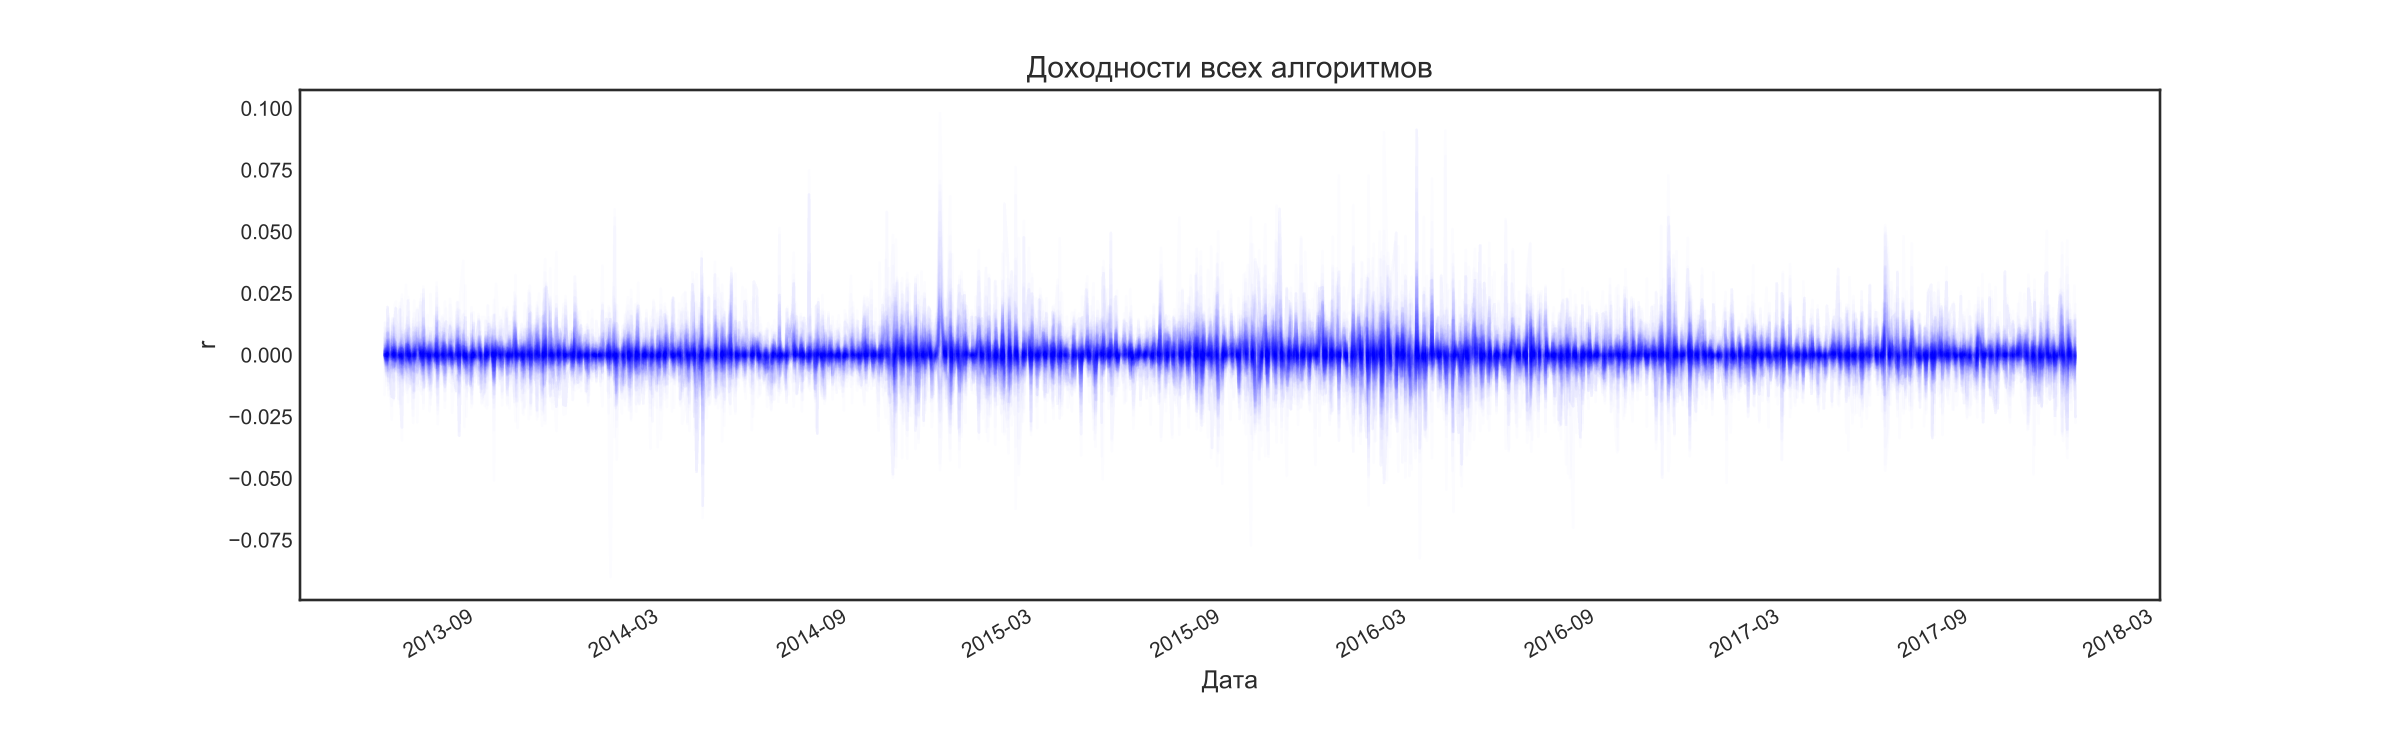
\includegraphics[width=\linewidth]{returns-all}
	\caption{Распределение доходностей во времени, на графике изображены доходности всех стратегий с наложением. На графике видна кластеризация волатильности, что позволяет говорить о наличии эффекта стохастической волатильности}
\end{figure}
\subsection{Распределение скользящих корреляций во времени}
\begin{figure}[h]
	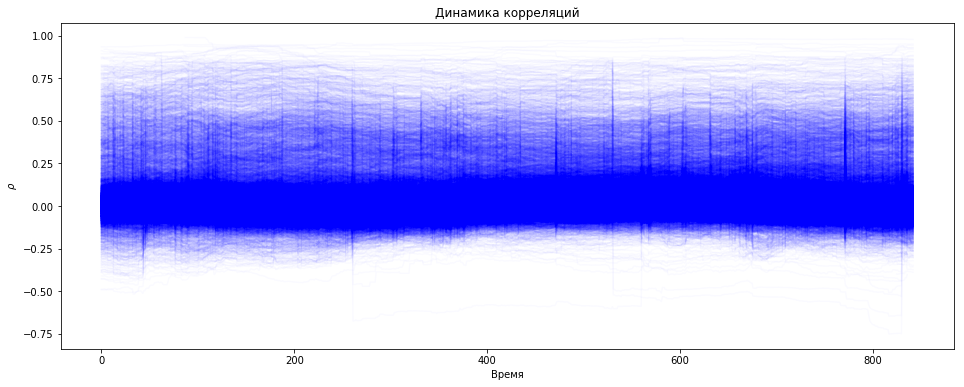
\includegraphics[width=\linewidth]{correlations}
	\caption{В отличие от результатов ранних исследований о динамике корреляций рыночных активов (гипотезы когерентности рынка), распределение скользящих корреляций во времени для торговых стратегий довольно стабильно}
\end{figure}
\end{document}